%% bare_jrnl.tex
%% V1.4b
%% 2015/08/26
%% by Michael Shell
%% see http://www.michaelshell.org/
%% for current contact information.
%%
%% This is a skeleton file demonstrating the use of IEEEtran.cls
%% (requires IEEEtran.cls version 1.8b or later) with an IEEE
%% journal paper.
%%
%% Support sites:
%% http://www.michaelshell.org/tex/ieeetran/
%% http://www.ctan.org/pkg/ieeetran
%% and
%% http://www.ieee.org/

%%*************************************************************************
%% Legal Notice:
%% This code is offered as-is without any warranty either expressed or
%% implied; without even the implied warranty of MERCHANTABILITY or
%% FITNESS FOR A PARTICULAR PURPOSE! 
%% User assumes all risk.
%% In no event shall the IEEE or any contributor to this code be liable for
%% any damages or losses, including, but not limited to, incidental,
%% consequential, or any other damages, resulting from the use or misuse
%% of any information contained here.
%%
%% All comments are the opinions of their respective authors and are not
%% necessarily endorsed by the IEEE.
%%
%% This work is distributed under the LaTeX Project Public License (LPPL)
%% ( http://www.latex-project.org/ ) version 1.3, and may be freely used,
%% distributed and modified. A copy of the LPPL, version 1.3, is included
%% in the base LaTeX documentation of all distributions of LaTeX released
%% 2003/12/01 or later.
%% Retain all contribution notices and credits.
%% ** Modified files should be clearly indicated as such, including  **
%% ** renaming them and changing author support contact information. **
%%*************************************************************************
\documentclass[journal, twoside, a4paper]{IEEEtran_LEEC_v1}
%
% *** CITATION PACKAGES ***
%
\usepackage{cite}
%
% *** GRAPHICS RELATED PACKAGES ***
%
\usepackage[pdftex]{graphicx}
%\usepackage[dvips]{graphicx}
%
\usepackage{amsmath}
%
% *** SPECIALIZED LIST PACKAGES ***
%
%\usepackage{algorithmic}
%
% *** ALIGNMENT PACKAGES ***
%
%\usepackage{array}
%
\usepackage{listings}
\usepackage{color}
\usepackage{caption}

\definecolor{codegreen}{rgb}{0,0.6,0}
\definecolor{codegray}{rgb}{0.5,0.5,0.5}
\definecolor{codepurple}{rgb}{0.58,0,0.82}
\definecolor{backcolour}{rgb}{0.95,0.95,0.92}

\lstdefinestyle{mystyle}{
	backgroundcolor=\color{backcolour},
	commentstyle=\color{codegreen},
	keywordstyle=\color{magenta},
	numberstyle=\tiny\color{codegray},
	stringstyle=\color{codepurple},
	basicstyle=\footnotesize,
	breakatwhitespace=false,
	breaklines=true,
	captionpos=t,
	keepspaces=true,
	numbers=left,
	numbersep=5pt,
	showspaces=false,
	showstringspaces=false,
	showtabs=false,
	tabsize=2
}
\lstset{style=mystyle}

%\DeclareCaptionStyle{listing} [justification=raggedright,indention=30pt, labelfont=bf]{}
%\captionsetup[lstlisting]{style=listing}

\renewcommand{\lstlistingname}{Listagem}
\renewcommand{\tablename}{Tabela}
\renewcommand{\refname}{Referências bilbiográficas}
\renewcommand{\appendixname}{Anexo}

% *** SUBFIGURE PACKAGES ***
%
\usepackage[caption=false,font=normalsize,labelfont=sf,textfont=sf]{subfig}
%
\usepackage[utf8]{inputenc}
%
\usepackage{url}
%
%--------------------------------------------------------------------------------------------
\begin{document}
%--------------------------------------------------------------------------------------------
\newcommand{\anoletivo}[1][]{2019/2020}
\newcommand{\nomealuno}[1][]{Nome aluno}
\newcommand{\numeroaluno}[1][]{33333}
\newcommand{\nomeorientador}[1][]{Nome Orientador}
\newcommand{\nomecoorientador}[1][]{Nome Coorientador}
\newcommand{\nomeprojeto}[1][]{Título do meu projeto}
\newcommand{\codigoprojeto}[1][]{P20--01}
\newcommand{\datasubmissao}[1][]{12 de julho de 2020}

%--------------------------------------------------------------------------------------------
\title{\codigoprojeto-\nomeprojeto}
%
%
% The paper headers
\markboth{Artigo de Projeto de 3ºano de Mestrado Integrado em Engenharia Eletrotécnica e de Computadores, \anoletivo}%
{\nomealuno~\MakeLowercase{\textit{et al.}}: \nomeprojeto}
%
\author{\nomealuno~(\numeroaluno),~\nomecoorientador~(UTAD/ECT),~\nomeorientador~(UTAD/ECT)% <-this % stops a space
\thanks{\nomeorientador  pertence ao Departamento de Engenharias da Escola de Ciências e Tecnologia da Universidade de Trás-os-Montes e Alto Douro e é Investigador Sénior do INESC-TEC (ver perfil ORCID em http://orcid.org/0000-0003-2440-915).}% <-this % stops a space
\thanks{Artigo submetido em \datasubmissao.}}
%
\IEEEpubid{
	\begin{minipage}
		{\textwidth}\ 
		\\[15mm] 
		\centering
		\codigoprojeto~\copyright~2020 UTAD/ECT
	\end{minipage}}
\IEEEpubidadjcol
%
\IEEEspecialpapernotice{(Para entregar no dia 12 de julho NÃO preencher o nome do aluno nem dos Orientadores (Blind review). Depois de efetuadas as corre\c cões que os professores mandarem fazer, deverá ser retirado o código do projeto no título, acrescentados os nomes do aluno e orientadores e apagada esta nota, passando o paper ao estado final. Entrega final obrigatória até ao dia 30 de julho.)}
%
% make the title area
\maketitle

%
% As a general rule, do not put math, special symbols or citations
% in the abstract or keywords.
\begin{abstract}
% Nota: Escrever o resumo em Inglês (máx. 150 palavras)
This is the \LaTeX template for the paper of the Project in Electrical and Computer Engineering. The article should not exceed 10 pages and should not be less than 6 pages. It should consist of an abstract (in English and Portuguese - maximum 150 words each) and three key words (in English and Portuguese). The structure of the paper should be composed at least by: Introduction, Development, Conclusions and References.
\end{abstract}
%
% Escolher as palavras chave mais importantes, que definam os termos de pesquisa para o vosso artigo!
% Máximo de 5 palavras-chave
%
\begin{IEEEkeywords}
IEEE, IEEEtran, journal, \LaTeX, template.
\end{IEEEkeywords}

%--------------------------------------------------------------------------------------------
\section{Introdução}
%--------------------------------------------------------------------------------------------
%
\IEEEPARstart{T}{his} demo file is intended to serve as a ``starter file''
for IEEE journal papers produced under \LaTeX\ using
IEEEtran.cls version 1.8b and later.

O artigo terá de ser elaborado em \LaTeX~\cite{Lamport}. Existem duas formas de o fazer: instalando um compilador dedicado ou usando um compilador online. Em (\url{https://www.overleaf.com/}) é disponibilizado um compilador e um editor online que lhe permitirá elaborar o artigo. Esta plataforma online permite também o trabalho colaborativo.

Para usar um compilador local, deverá instalar o MikTeX (\url{http://miktek.org}) e depois instalar um editor dedicado ao \LaTeX. Embora o \LaTeX seja compilado e, por isso, pode ser editado num editor de texto (ex. Notepad), aconselha-se o uso de um editor dedicado. Existem vários editores para \LaTeX para sistemas Windows (ex. TeXstudio, WinEdt, LEd, Texmaker, entre outros) e para Linux (ex. Kile, Texmaker, entre outros). Em Engenharia Electrotécnica e de Computadores, de momento, é mais utilizado o TeXstudio (\url{http://texstudio.sourceforge.net/}) disponível para as plataformas Windows, Linux e Mac OS X.

Depois de instalado o software edite o ficheiro \verb"ArtigoLEECv1.tex", altere o conteúdo do texto e compile usando PDFLaTeX~\cite{Bay1}.

Nas próximas secções estão alguns exemplos do uso de equações, figuras e tabelas. Os exemplos usados abrangem uma diversidade de situações sendo abordadas quase tudo o que será necessário para a elaboração do artigo. De qualquer modo, existe uma enorme quantidade de informação sobre \LaTeX na internet (por razões óbvias não utilize nos motores de busca a expressão ``latex'' sozinha mas sim acompanhada de uma outra palavra que necessite, ex: ``latex table'' para pesquisar como elaborar tabelas em \LaTeX).

\subsection{Título de uma subsecção}
As subsecções devem ser usadas em número maior do que um.

\subsubsection{Título de uma sub-subsecção}
As subsecções devem ser usadas em número maior do que um.


% An example of a floating figure using the graphicx package.
% Note that \label must occur AFTER (or within) \caption.
% For figures, \caption should occur after the \includegraphics.
% Note that IEEEtran v1.7 and later has special internal code that
% is designed to preserve the operation of \label within \caption
% even when the captionsoff option is in effect. However, because
% of issues like this, it may be the safest practice to put all your
% \label just after \caption rather than within \caption{}.
%
% Reminder: the "draftcls" or "draftclsnofoot", not "draft", class
% option should be used if it is desired that the figures are to be
% displayed while in draft mode.
%
%\begin{figure}[!t]
%\centering
%\includegraphics[width=2.5in]{myfigure}
% where an .eps filename suffix will be assumed under latex, 
% and a .pdf suffix will be assumed for pdflatex; or what has been declared
% via \DeclareGraphicsExtensions.
%\caption{Simulation results for the network.}
%\label{fig_sim}
%\end{figure}

% Note that the IEEE typically puts floats only at the top, even when this
% results in a large percentage of a column being occupied by floats.


% An example of a double column floating figure using two subfigures.
% (The subfig.sty package must be loaded for this to work.)
% The subfigure \label commands are set within each subfloat command,
% and the \label for the overall figure must come after \caption.
% \hfil is used as a separator to get equal spacing.
% Watch out that the combined width of all the subfigures on a 
% line do not exceed the text width or a line break will occur.
%
\begin{figure*}[!t]
	\centering
	\subfloat[Case I]{
\includegraphics[width=2.5in]{Figure.jpg}%
	\label{fig_first_case}}
	\hfil
	\subfloat[Case II]{
\includegraphics[width=2.5in]{Figure.jpg}%
	\label{fig_second_case}}
	\caption{Simulation results for the network.}
	\label{fig_sim}
\end{figure*}
%
% Note that often IEEE papers with subfigures do not employ subfigure
% captions (using the optional argument to \subfloat[]), but instead will
% reference/describe all of them (a), (b), etc., within the main caption.
% Be aware that for subfig.sty to generate the (a), (b), etc., subfigure
% labels, the optional argument to \subfloat must be present. If a
% subcaption is not desired, just leave its contents blank,
% e.g., \subfloat[].


% An example of a floating table. Note that, for IEEE style tables, the
% \caption command should come BEFORE the table and, given that table
% captions serve much like titles, are usually capitalized except for words
% such as a, an, and, as, at, but, by, for, in, nor, of, on, or, the, to
% and up, which are usually not capitalized unless they are the first or
% last word of the caption. Table text will default to \footnotesize as
% the IEEE normally uses this smaller font for tables.
% The \label must come after \caption as always.
%
%\begin{table}[!t]
%% increase table row spacing, adjust to taste
%\renewcommand{\arraystretch}{1.3}
% if using array.sty, it might be a good idea to tweak the value of
% \extrarowheight as needed to properly center the text within the cells
%\caption{An Example of a Table}
%\label{table_example}
%\centering
%% Some packages, such as MDW tools, offer better commands for making tables
%% than the plain LaTeX2e tabular which is used here.
%\begin{tabular}{|c||c|}
%\hline
%One & Two\\
%\hline
%Three & Four\\
%\hline
%\end{tabular}
%\end{table}


% Note that the IEEE does not put floats in the very first column
% - or typically anywhere on the first page for that matter. Also,
% in-text middle ("here") positioning is typically not used, but it
% is allowed and encouraged for Computer Society conferences (but
% not Computer Society journals). Most IEEE journals/conferences use
% top floats exclusively. 
% Note that, LaTeX2e, unlike IEEE journals/conferences, places
% footnotes above bottom floats. This can be corrected via the
% \fnbelowfloat command of the stfloats package.

%--------------------------------------------------------------------------------------------
\section{Desenvolvimento}
%--------------------------------------------------------------------------------------------
Nesta secção deve ser apresentado o estado da arte ou trabalho realizado por outros autores que estejam de base ou sustentem o trabalho apresentado. O título desta secção pode ser relacionado com o tema do trabalho. Por exemplo, \textbf{redes de sensores} poderia ser um nome onde se discute este tipo de implementações.

Utilize linguagem própria e procure alguém para rever o ser artigo para este ser claro e sem erros. Não utilize expressões brasileiras (ex: resistor, capacitor, entre outras), evite o uso de items (em  ambiente \LaTeX \texttt{itemize}), evite o \textit{copy}-\textit{paste} (plágio) pois será utilizado um \textit{software} que procurará na internet por expressões idênticas (\textit{software} anti-plágio). Aos artigos que estiverem nessa situação será atribuída a classificação de 0 (zero valores).

Segue-se um exemplo da utilização de uma equação:
\begin{equation}
	\frac{-b\pm\sqrt{b^2-4ac}}{2a}
	\label{eq:Resolvente}
\end{equation}

Bem como a referência à equação anterior. Na equação (\ref{eq:Resolvente}) foi abordada a resolução de uma equação de segundo grau. A equação seguinte refere-se à utilização de integrais.

\begin{equation}
\phi_n(\kappa) =
\frac{1}{4\pi^2\kappa^2} \int_0^\infty
\frac{\sin(\kappa R)}{\kappa R}
\frac{\partial}{\partial R}
\left[R^2\frac{\partial D_n(R)}{\partial R}\right]\,dR	
\label{eq:Integral}
\end{equation}

Nesta equação aborda-se a utilização de chavetas:
\begin{equation}
f(x) =
\begin{cases}
1 				& -1 \le x < 0 \\
\frac{1}{2} & x = 0 \\
1 - x^2 & \mbox{outros}
\end{cases}
\label{eq:Chavetas}
\end{equation}

A utilização de figuras é essencial num artigo, quer sejam esquemas, quer sejam diagramas ou até fotografias~\cite{Swa82}. Faça, sempre que possível as suas figuras, caso não seja possível refira sempre a sua fonte. Neste modelo poderá utilizar figuras, JPG ou PNG. Use JPG para fotografias e PNG para desenhos e esquemas. Para uma melhor qualidade sugiro a utilização do CorelDraw para o desenvolvimento das figuras (esquemas e/ou diagramas) e exportar para PNG~\cite{Ta}. Para esquemas desenvolvidos no Eagle, exporta-se para EPS (Cam Processor) e depois converte-se para PNG utilizando, por exemplo, o CorelDraw.

\begin{figure}[ht]
	%
\includegraphics[width=\columnwidth]{Figure.jpg}
	
\includegraphics[width=80mm]{Figure.jpg}
	\caption{Exemplo de uma figura}
	\label{fig:ExemploFigura}
\end{figure}

Embora não muito usuais as tabelas podem ser uma boa forma de representar os resultados. A Tab.~\ref{tab:ExemploTabela1} é um exemplo de utilização de uma tabela para representar resultados, neste caso classificação dos alunos num teste. Outro tipo de tabelas pode ser consultado na internet usando ``latex table'' como expressão de pesquisa.

\begin{table}[ht]
	\caption{Exemplo de uma tabela}
	\label{tab:ExemploTabela1}
	\centering
	\begin{tabular}{lcc}
		\hline
		\multicolumn{1}{c}{\bf Aluno} & \bf Número & \bf Teste\\
		\hline
		\hline
		Mário Freitas & 1234 & 9.45\\
		Luís Freitas & 1234 & 9.45\\
		Manuel Freitas & 1234 & 9.45\\
		António Freitas & 1234 & 9.45\\
		\hline
		
	\end{tabular}
\end{table}

%--------------------------------------------------------------------------------------------
\section{Protótipo}
%--------------------------------------------------------------------------------------------
Se conveniente, uma secção que apresente a implementação efetuada no decorrer do projeto. Poderá ser uma implementação em hardware (um circuito eletrónico, uma placa, uma montagem), onde se descreve o circuito elétrico, onde se apresenta um diagrama de blocos, etc., ou uma implementação em software, onde se apresenta um fluxograma, algoritmo, listagem, etc.

Consoante o tipo de projeto, poderá existir nesta secção algo de discussão sobre esta implementação.

Normalmente existe também a necessidade de apresentar código nos artigos, como por exemplo a seguinte Listagem~\ref{codigo}.


\begin{lstlisting}[language=Java,caption={Exemplo de um código Java},label={codigo}]
package com.javadb.examples;

import java.util.Arrays;
import java.util.List;
import java.util.Iterator;

public class Main {

	public static void main(String[] args) {

		String[] array = {"Programming", "is", "fun"};
		List<String> list = Arrays.asList(array);
	
		Iterator<String> iterator = list.iterator();
		while (iterator.hasNext()) {
			System.out.println(iterator.next());
		}
	}
}
\end{lstlisting}

%--------------------------------------------------------------------------------------------
\section{Resultados e discussão}
%--------------------------------------------------------------------------------------------
Secção onde se mostram os resultados obtidos durante a execução do projeto, apresentando igualmente uma discussão crítica dos mesmos. Algo onde o aluno teça considerações práticas sobre a suma implementação: O que poderia ser melhor, o que correu menos bem, etc. Tudo deve ser reportado no artigo.

%--------------------------------------------------------------------------------------------
\section{Conclusões}
%--------------------------------------------------------------------------------------------

Nesta secção serão abordadas as conclusões do artigo. No entanto, e como falta ainda explicar com se faz a bibliografia, aproveito este espaço para fazê-lo. Toda a bibliografia a colocar deverá ser colocada num ficheiro à parte com extensão BIB (ex: \verb"MyProjLEECBibliography.bib" utilizado neste modelo). Nas vossas pesquisas utilizando a B-on poderão exportar a informação de um determinado artigo para BibTex e inserir essa informação no vosso ficheiro .BIB (trata-se de um ficheiro de texto que se pode editar no TeXstudio ou noutro editor de texto - ex: Notepad). Ao editarem esse ficheiro poderão reparar que o primeiro campo de cada entrada é uma referência (no caso do ficheiro \verb"MyProjLEECBibliography.bib" uma das entradas BOOK tem a referência Hale - neste caso é o último nome do autor mas não é obrigatório, é simplesmente mais fácil de se perceber no texto). No vosso documento .TEX (ex: este ficheiro) no local onde desejam colocar a citação inserem \verb"~\cite{referência}" (neste exemplo \verb"~\cite{Hale}").

Espero que este documento/modelo seja suficientemente explicativo para a elaboração correcta do artigo para a Unidade Curricular de Projecto em Engenharia Electrotécnica e de Computadores. Façam uma utilização correcta deste ficheiro e elaborem artigos cuidados e de excelente qualidade. O esforço e a excelência serão sempre recompensados.


% if have a single appendix:
%\appendix[Proof of the Zonklar Equations]
% or
%\appendix  % for no appendix heading
% do not use \section anymore after \appendix, only \section*
% is possibly needed

% use appendices with more than one appendix
% then use \section to start each appendix
% you must declare a \section before using any
% \subsection or using \label (\appendices by itself
% starts a section numbered zero.)
%

\appendices
\section{Demonstração da equação de Zonklar}
Inserir o texto da demonstração.

% you can choose not to have a title for an appendix
% if you want by leaving the argument blank
\section{}
Inserir o texto do Anexo.

% use section* for acknowledgment
\section*{Agradecimentos}

Os autores agradecem à empresa X os meios colocados à disposição e que permitiram levar o trabalho apresentado à fase atual de desenvolvimento.

%
%--------------------------------------------------------------------------------------------
% references section
%
\bibliographystyle{IEEEtran}
\bibliography{MyProjLEECBibliography}
%
% <OR> manually copy in the resultant .bbl file
% set second argument of \begin to the number of references
% (used to reserve space for the reference number labels box)

%\begin{thebibliography}{1}

%\bibitem{IEEEhowto:kopka}
%H.~Kopka and P.~W. Daly, \emph{A Guide to \LaTeX}, 3rd~ed.\hskip 1em plus
%  0.5em minus 0.4em\relax Harlow, England: Addison-Wesley, 1999.

%\end{thebibliography}
%
%--------------------------------------------------------------------------------------------
% biography section
% 
\newpage

\begin{IEEEbiography}[{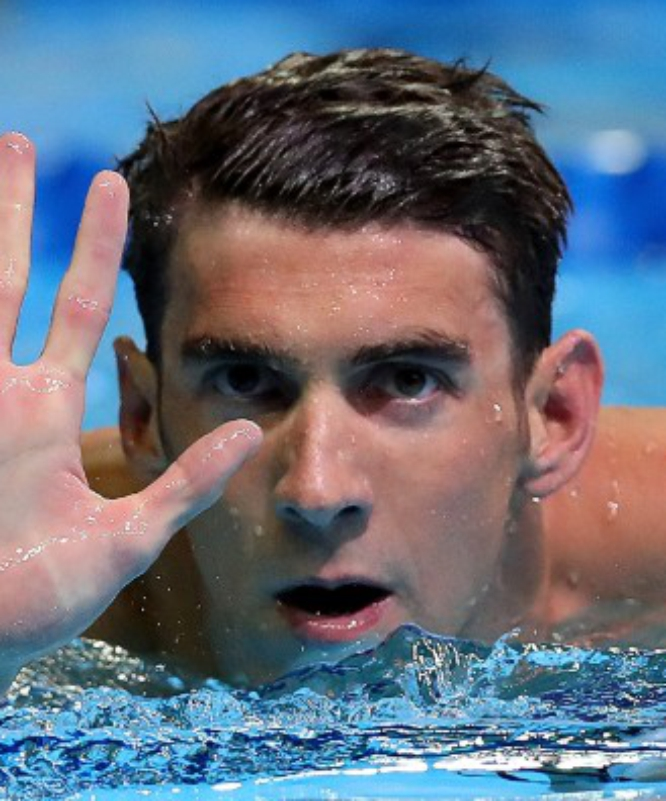
\includegraphics[width=1in,height=1.25in,clip,keepaspectratio]{Phelps.jpg}}]{Raul Morais dos Santos}
licenciou-se em Engenharia Electrotécnica (Ramo de Electrónica, Instrumentação e Computação), pela Universidade de Trás-os-Montes e Alto Douro (UTAD), Portugal, em 1993. Obteve o grau de Mestre em Electrónica Industrial pela Universidade do Minho, em 1998. O seu doutoramento, em Engenharia Electrotécnica e de Computadores, especialidade de microeletrónica, foi obtido na UTAD, em 2004. A sua Agregação em Engenharia Electrotécnica e de Computadores foi obtida na UTAD em 2009. Atualmente é Professor Associado com Agregação no Departamento de Engenharias da Escola de Ciências e Tecnologia da UTAD. As suas principais áreas de interesse incluem: sensores e interfaces sensoriais em microeletrónica, técnicas de recolha de energia para alimentação de dispositivos eletrónicos e redes de sensores sem fios em contextos de agricultura/viticultura de precisão. Tem também interesses no campo dos dispositivos biomédicos implantáveis, em particular nos sistemas de biotelemetria e nos microgeradores vibracionais para produção de energia no interior de dispositivos implantáveis. É atualmente membro integrado no Instituto de Engenharia de Sistemas e Computadores do Porto (INESC).
\end{IEEEbiography}

\begin{IEEEbiography}{Nome do aluno}
Biography text here.
\end{IEEEbiography}

% Sem fotografia
\begin{IEEEbiographynophoto}{John Doe}
Biography text here.
\end{IEEEbiographynophoto}

\vfill
%--------------------------------------------------------------------------------------------
\end{document}
%--------------------------------------------------------------------------------------------

